\subsection{ID3 algorithm}
We now know about the core concepts and components for building decision trees. The following algorithm introduces a standard procedure to build decision trees. 

ID3, short for \textbf{iterative Dicchotomiser 3}, was developed by Ross Quinlan in 1986 and is a predecessor of algorithms like C4.5. The key idea is the following:\sidenote{ID3}
\begin{enumerate}
  \item Calculate the entropy of every attribute using the data set $D$.
  \item Split the set $D$ into subsets using the attribute with the minimal resulting entropy.
  \begin{itemize}
    \item Meant is the entropy after splitting using this attribute.
    \item Equivalent formulation: choose the attribute maximizing the information gain.
  \end{itemize}
  \item Make a decision tree node containing that attribute.
  \item Recurse on the subsets using the remaining attributes.
\end{enumerate}

More formally, the algorithm looks as follows in pseudocode. We will afterward investigate certain details of the algorithm \ref{lst:3_id3}.

\begin{figure}[h]
\begin{lstlisting}[
  style=pseudocode, morekeywords={Require, if, then, else, for, each, do make, return},
  caption={ID3 algorithm code}, captionpos=b,
  label=lst:3_id3
]
Require: set of descriptive features $\mathbf{d}$
Require: set of training instances $\mathcal{D}$

// Different reasons to stop
if all instances in $\mathcal{D}$ have the same target level $C$ then
  return DecisionTree(leaf_node with label $C$)
else if $\mathbf{d}$ is empty then
  return DecisionTree(leaf_node with the label of majority target level in $\mathcal{D}$)
else if $\mathcal{D}$ is empty then
  return DecisionTree(leaf_node with label of the majority target level of the immediate parent node)

else
  // Pick feature
  $\mathbf{d}[best]\leftarrow \arg\max_{d\in \mathbf{d}} IG(d, \mathcal{D})$
  make a new node $Node_{\mathbf{d}[best]}$ and label it with $\mathbf{d}[best]$
  partition $\mathcal{D}$ using $\mathbf{d}[best]$
  remove $\mathbf{d}[best]$ from $\mathbf{d}$

  // Create subproblems
  for each partition $\mathcal{D}_i$ of $\mathcal{D}$ do
    grow a branch from $Node_{\mathbf{d}[best]}$ to the decision tree created by rerunning ID3 with $\mathcal{D} = \mathcal{D}_i$
\end{lstlisting}
\end{figure}

\begin{itemize}
  \item Detail 1: three different reasons to stop
  \begin{itemize}
    \item All instances have the same classification (labeled with consensus value)
    \item No features are left (labeled with majority value)
    \item Data set is empty (labeled with the majority value of the parent node)
  \end{itemize}
  \item Detail 2: which feature to select
  \begin{itemize}
    \item The feature should be picked that maximizes the information gain. 
    \item A feature can't be picked more than once along the path from the root.
  \end{itemize}
  \item Detail 3: subproblems are created based on the selected feature, building the decision tree in a divide-and-conquer fashion.
  \begin{itemize}
    \item The amount of subproblems is dependent on the selected feature.
  \end{itemize}
\end{itemize}

The ID3 algorithm has a lot of variations, from which we're gonna take a look at some.

\subsubsection*{Alternative information gain notions}
Information gain ($IG$) aims to measure the improvement in purity, predictability, and compressibility. Instead, it is also possible to select a feature maximizing:
\begin{itemize}
  \item The information gain ratio ($GR$), or
  \item The Gini index ($Gini$)
\end{itemize}

The standard information gain notion favors features with many values since a split in many subsets increases the entropy. The \textbf{information gain ratio}\sidenote{Information gain ratio $GR$} on the other hand addresses:
\begin{align*}
  GR(d, \mathcal{D}) = \underbrace{\frac{IG(d, \mathcal{D})}{-\sum_{l\in levels(d)} \Pr[d=l]\cdot\log_2(\Pr[d=l])}}_{\text{\color{gray}Basically: make absolute value relative}}
\end{align*}

Another alternative is the \textbf{Gini index}\sidenote{Gini index $Gini$} measuring impurity in an alternative way. Specifically, it uses the expected misclassification rate when guessing based on the observed distribution:
\renewcommand{\arraystretch}{0.6}
\begin{align*}
  Gini(t,\mathcal{D}) = \underbrace{1-\sum_{l\in levels(t)}\underbrace{\Pr[t=l]^2}_{\begin{array}{c}
    \scriptstyle\text{\color{gray}Guess } t=l \text{ \color{gray} with probability } \Pr[t=l] \text{ \color{gray} and}\\
    \scriptstyle\text{\color{gray}with probability}  \Pr[t=l] \text{ \color{gray} this is right}
  \end{array}}}_{\text{\color{gray}Probability of guessing the wrong label}}
\end{align*}
\renewcommand{\arraystretch}{1} 

A comparison of all the evaluation metrics can be found in figure \ref{fig:3_id3_alternative_evaluation}.

\begin{figure}[h]
  \centering
  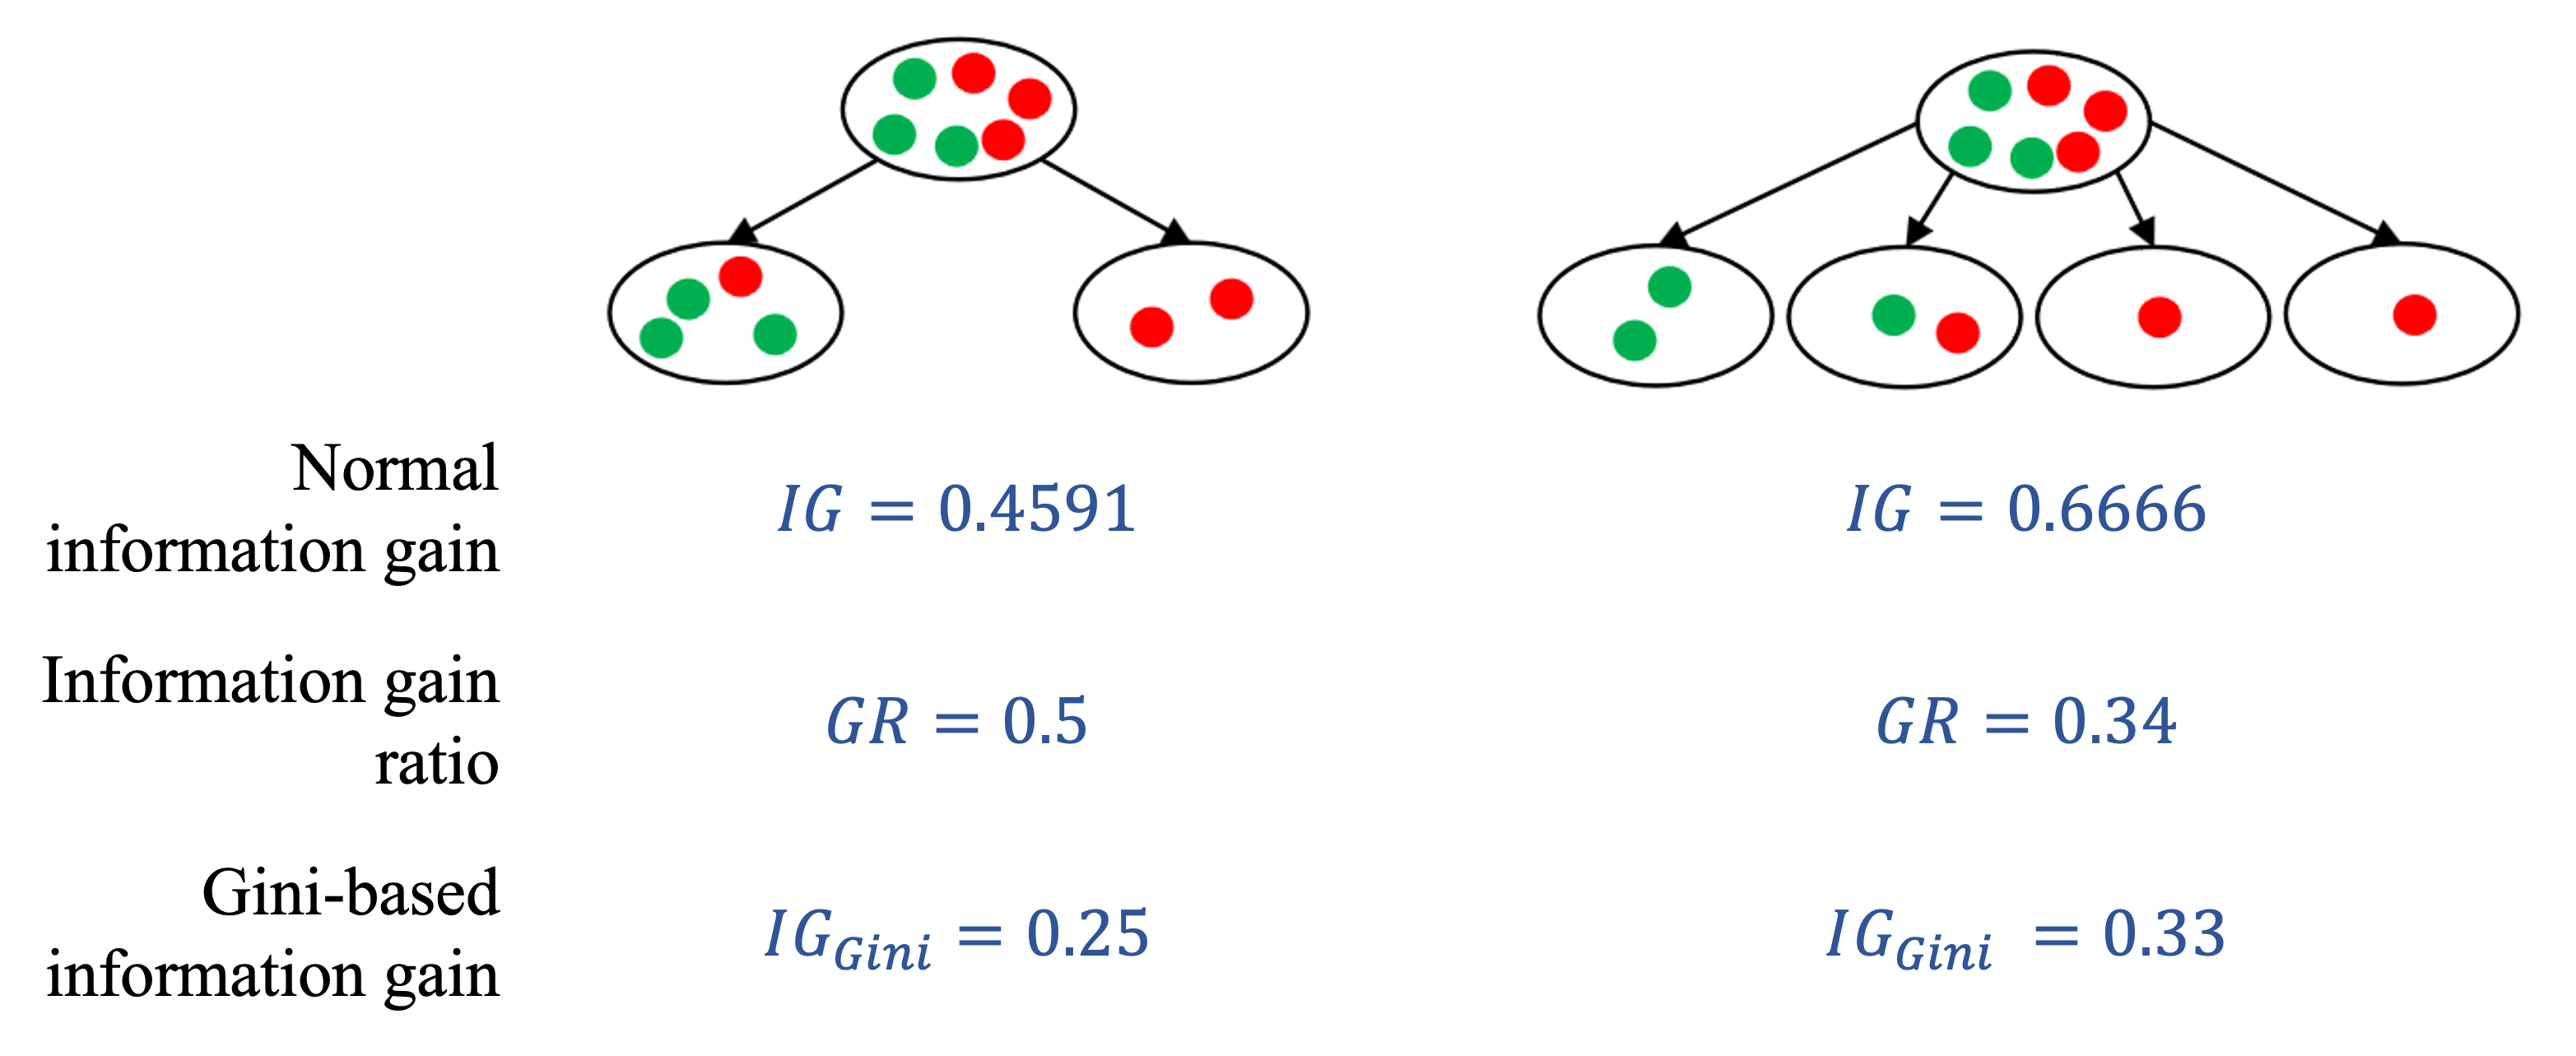
\includegraphics[width=0.9\textwidth]{assets/trees/id3/comp_evaluation_metrics.png}
  \caption{Comparison of $IG$, $GR$, and $Gini$}
  \label{fig:3_id3_alternative_evaluation}
\end{figure}


\subsubsection*{Pruning decision trees}
When applying the ID3-algorithm to build decision trees, two possible problems can occur:
\begin{itemize}
  \item The decision tree overfits the data.
  \item The decision tree is too complex or deep.
\end{itemize}
For those problems, there are now two solution directions:
\begin{itemize}
  \item Pre-pruning, so an early stopping, functioning forwards, and
  \item Post-pruning, so a reduced error, functioning backward.
\end{itemize}

We'll first take a deeper look into \textbf{pre-pruning}\sidenote{Pre-pruning}, where at some point the procedure of creating subtrees is \textbf{stopped} at which point the label is determined via majority vote. There are many possible stopping criteria, for example:
\begin{itemize}
  \item Lower bound on number of instances.
  \item Lower bound for information gain.
\end{itemize}
The trees resulting from pre-pruning may not be consistent with respect to the data. But they generalize and therefore avoid overfitting nicely. So the procedure is very efficient, but strong dependencies at lower levels of the tree might be missed.

Next, let's investigate \textbf{post-pruning}\sidenote{Post-pruning}, where first the whole decision tree is built and then some branches are \textbf{cut-off} that don't add too much information. One common approach for cutting off is to
\begin{itemize}
  \item First split the data in a \textbf{training set} and a \textbf{validation/test set}, 
  \item Built the decision tree based on the training set, and then
  \item Measure the performance of each split based on the validation/test set (e.g., count misclassified instances).
\end{itemize}

\subsubsection*{Ensembles}

The final extension works with \textbf{ensembles}\sidenote{Ensembles}, where:
\begin{itemize}
  \item Instead of creating a single decision tree, a set of trees called a "model ensemble" is created.
  \item The models should complement each other.
  \item Different models can then "vote" on a label (votes may be weighted).
\end{itemize}

The concept relates to the "wisdom of the crowds" and aims at avoiding overfitting. The multiple trees may give different answers. Multiple trees can give different answers, then a "compromise" should be found, so the most frequent value or average is selected. There are many variations of this idea.

The first implementation of ensembles is called \textbf{boosting}\sidenote{Boosting} where an iterative correction in a sequential manner happens. 
\begin{itemize}
  \item This correction happens by changing the data set based on previous misclassifications.
  \item Instances that were wrongly classified get a higher weight for training the next model.
  \item This creates a sequence of models, that combined lead to a (rater) correct classification.
\end{itemize}

The second implementation is called \textbf{bagging}\sidenote{Bagging} where data is split upfront allowing a parallel rather than sequential model training. We alter the original data set by adjusting the rows (so the instances).
\begin{itemize}
  \item Each model is based on a random sample of the data set.
  \item The idea is, that models are avoided depending on a specific sample in the data set. This is supposed to avoid that learning in decision trees is very sensitive to small variations.
  \item How the training bags are created has a lot of variants. Instances can for example be removed, or other duplicated, etc.
\end{itemize}

A third implementation called \textbf{subspace sampling}\sidenote{Subspace sampling} takes a similar approach as bagging, but instead of altering the rows, the columns so the features are adjusted.
\begin{itemize}
  \item Each model is based on a random set of descriptive features.
  \item The idea is that overfitting is less likely and also the training process is faster when focussed on just a few features instead of the whole feature space.
  \item The similarity to (instance) bagging is highlighted with the alternative name "feature bagging".
\end{itemize}

A fourth implementation combines feature and instance bagging and is called \textbf{random forest}\sidenote{Random forest}. All three bagging strategies are also visualized in \ref{fig:3_bagging}.

\begin{figure}[h]
  \centering
  \begin{subfigure}{0.3\textwidth}
    \centering
    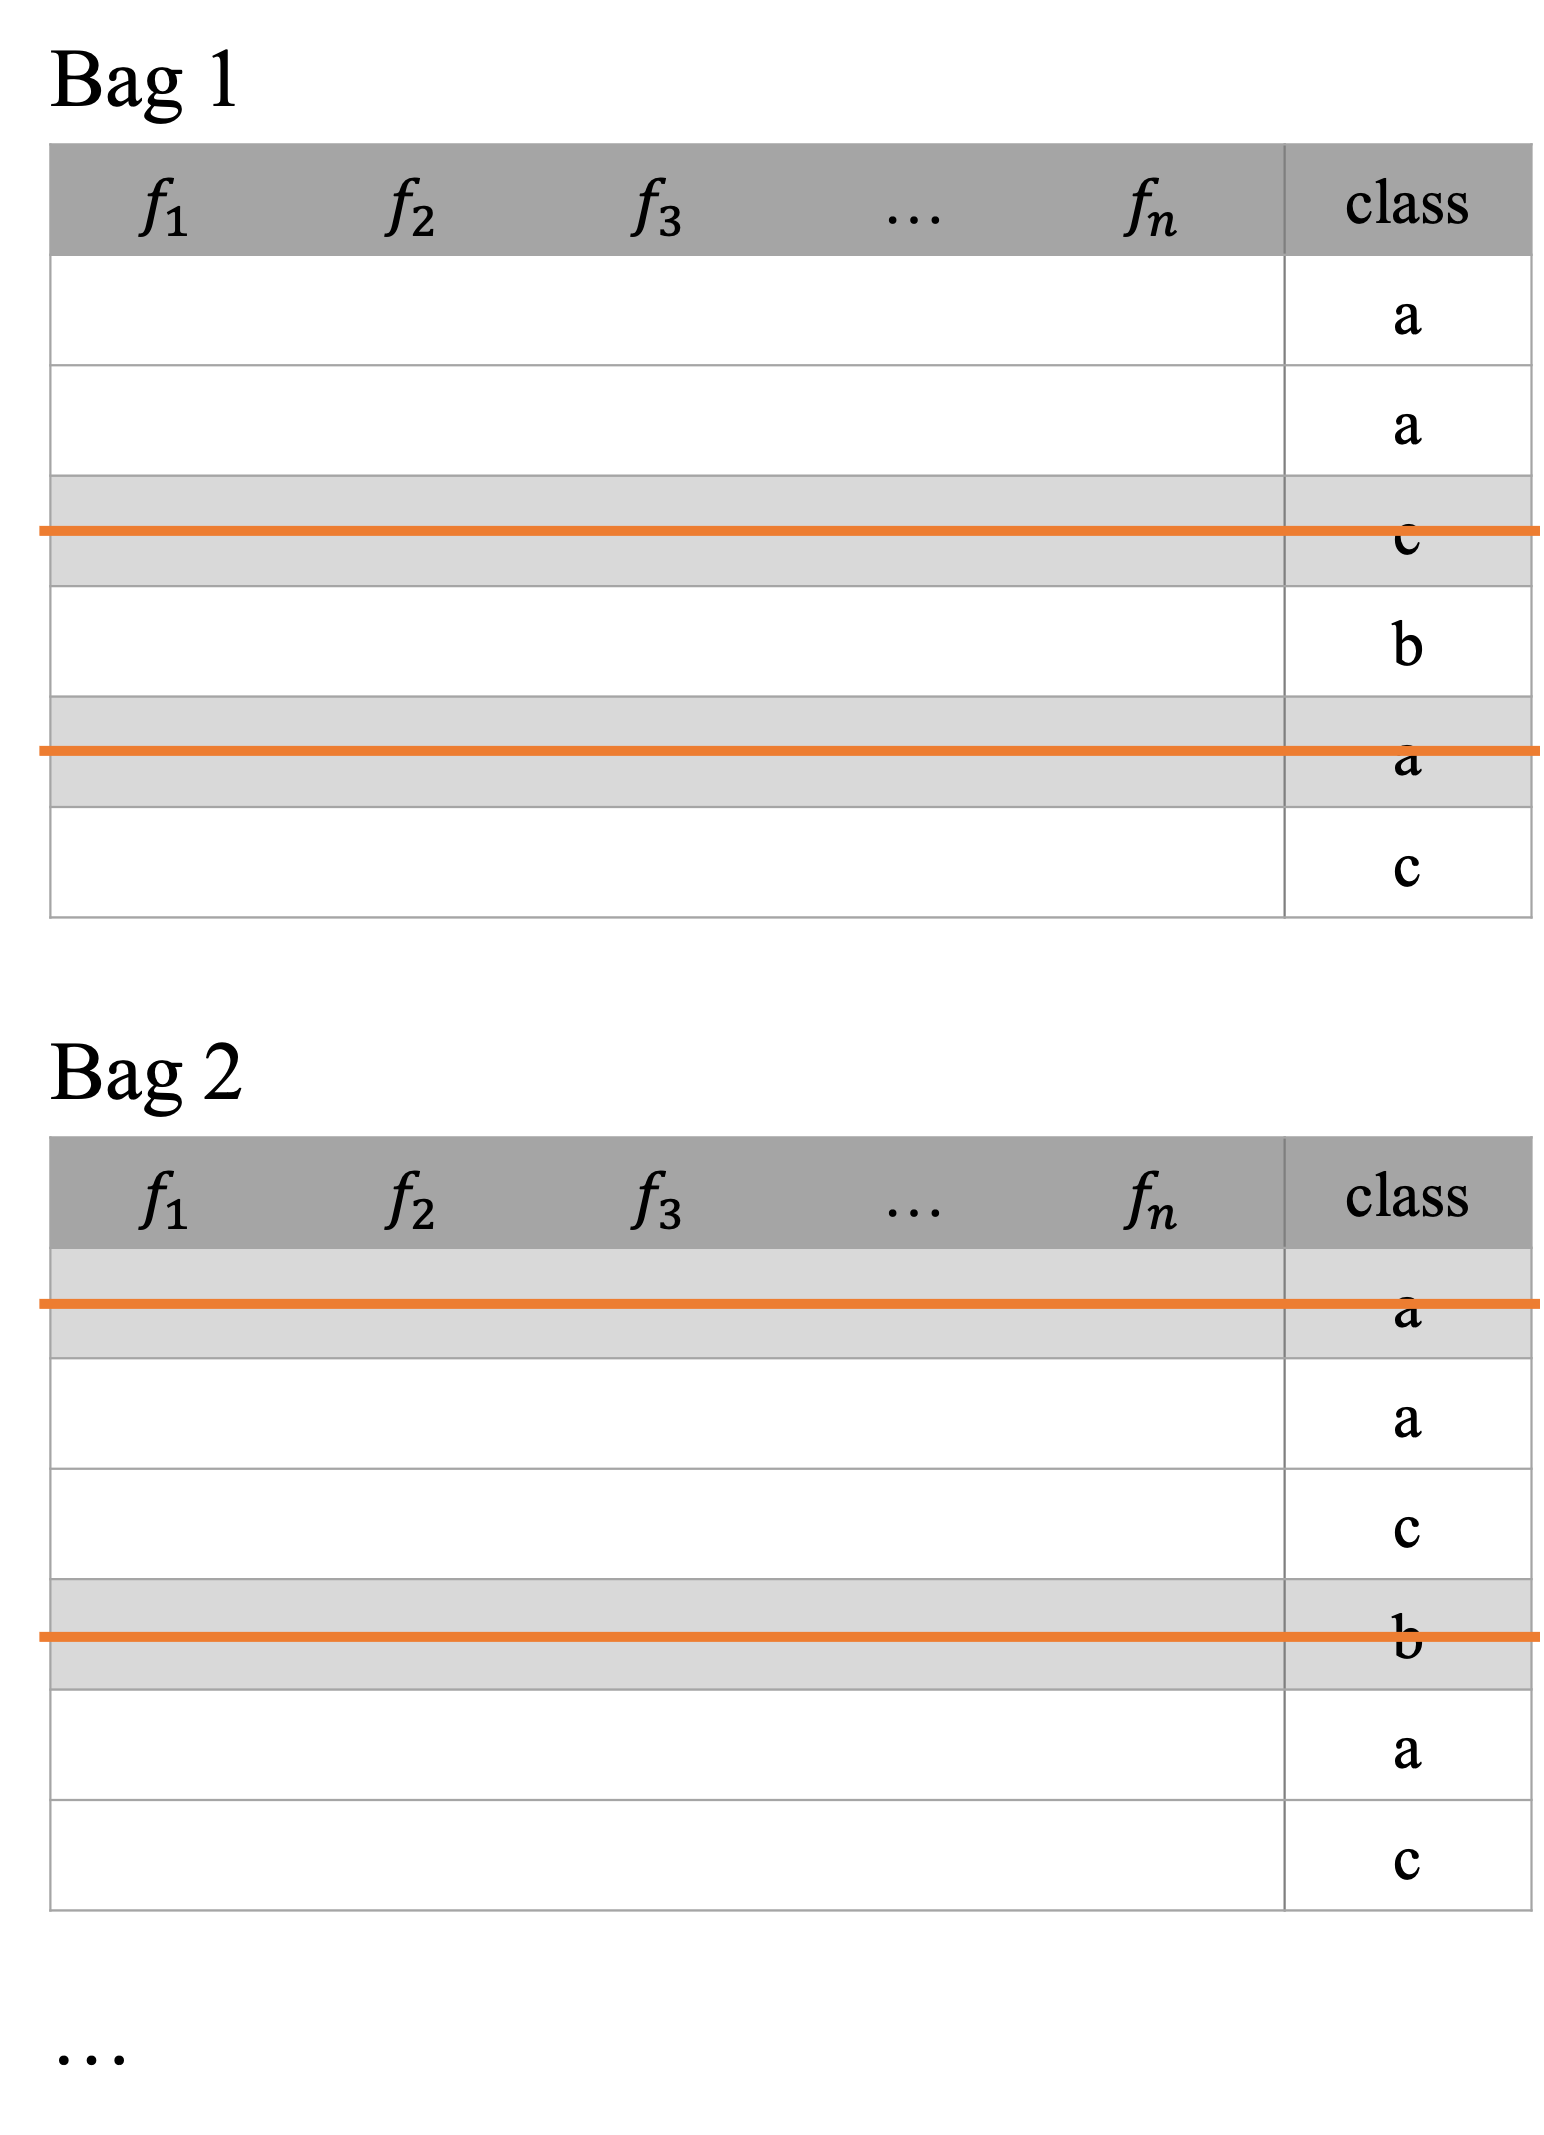
\includegraphics[width=0.9\textwidth]{assets/trees/id3/ensemble_instance_bagging.png}
    \subcaption{(Instance) bagging}
  \end{subfigure}
  \begin{subfigure}{0.3\textwidth}
    \centering
    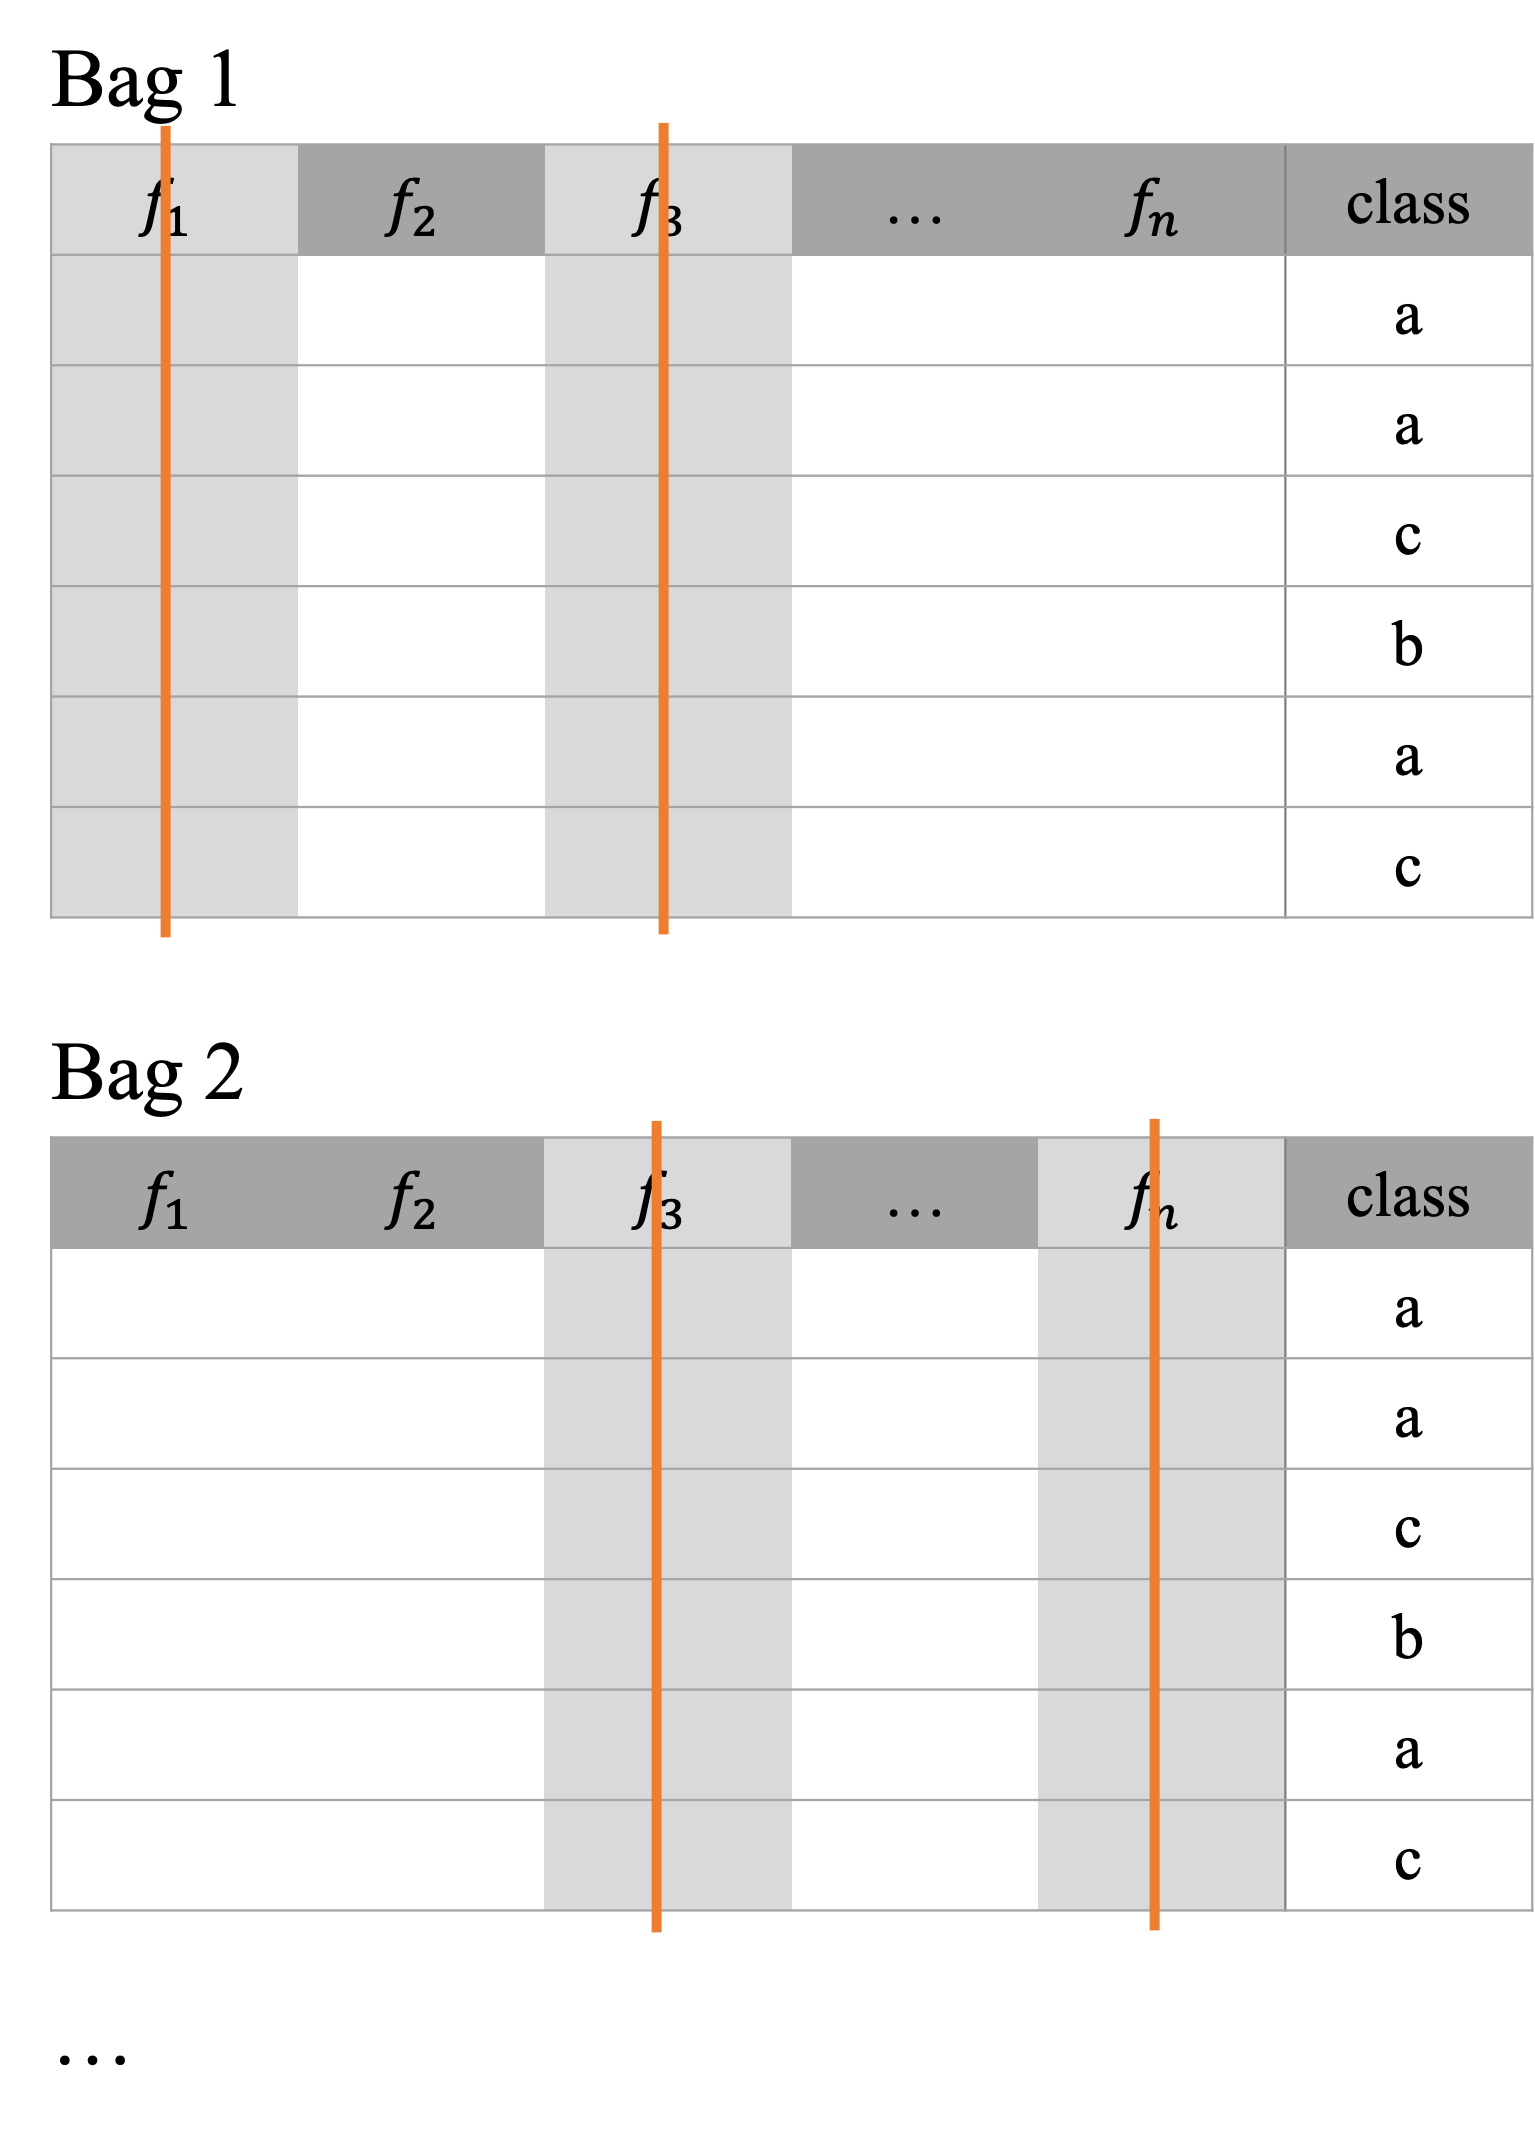
\includegraphics[width=0.9\textwidth]{assets/trees/id3/ensemble_feature_bagging.png}
    \subcaption{Subspace sampling (feature bagging)}
  \end{subfigure}
  \begin{subfigure}{0.3\textwidth}
    \centering
    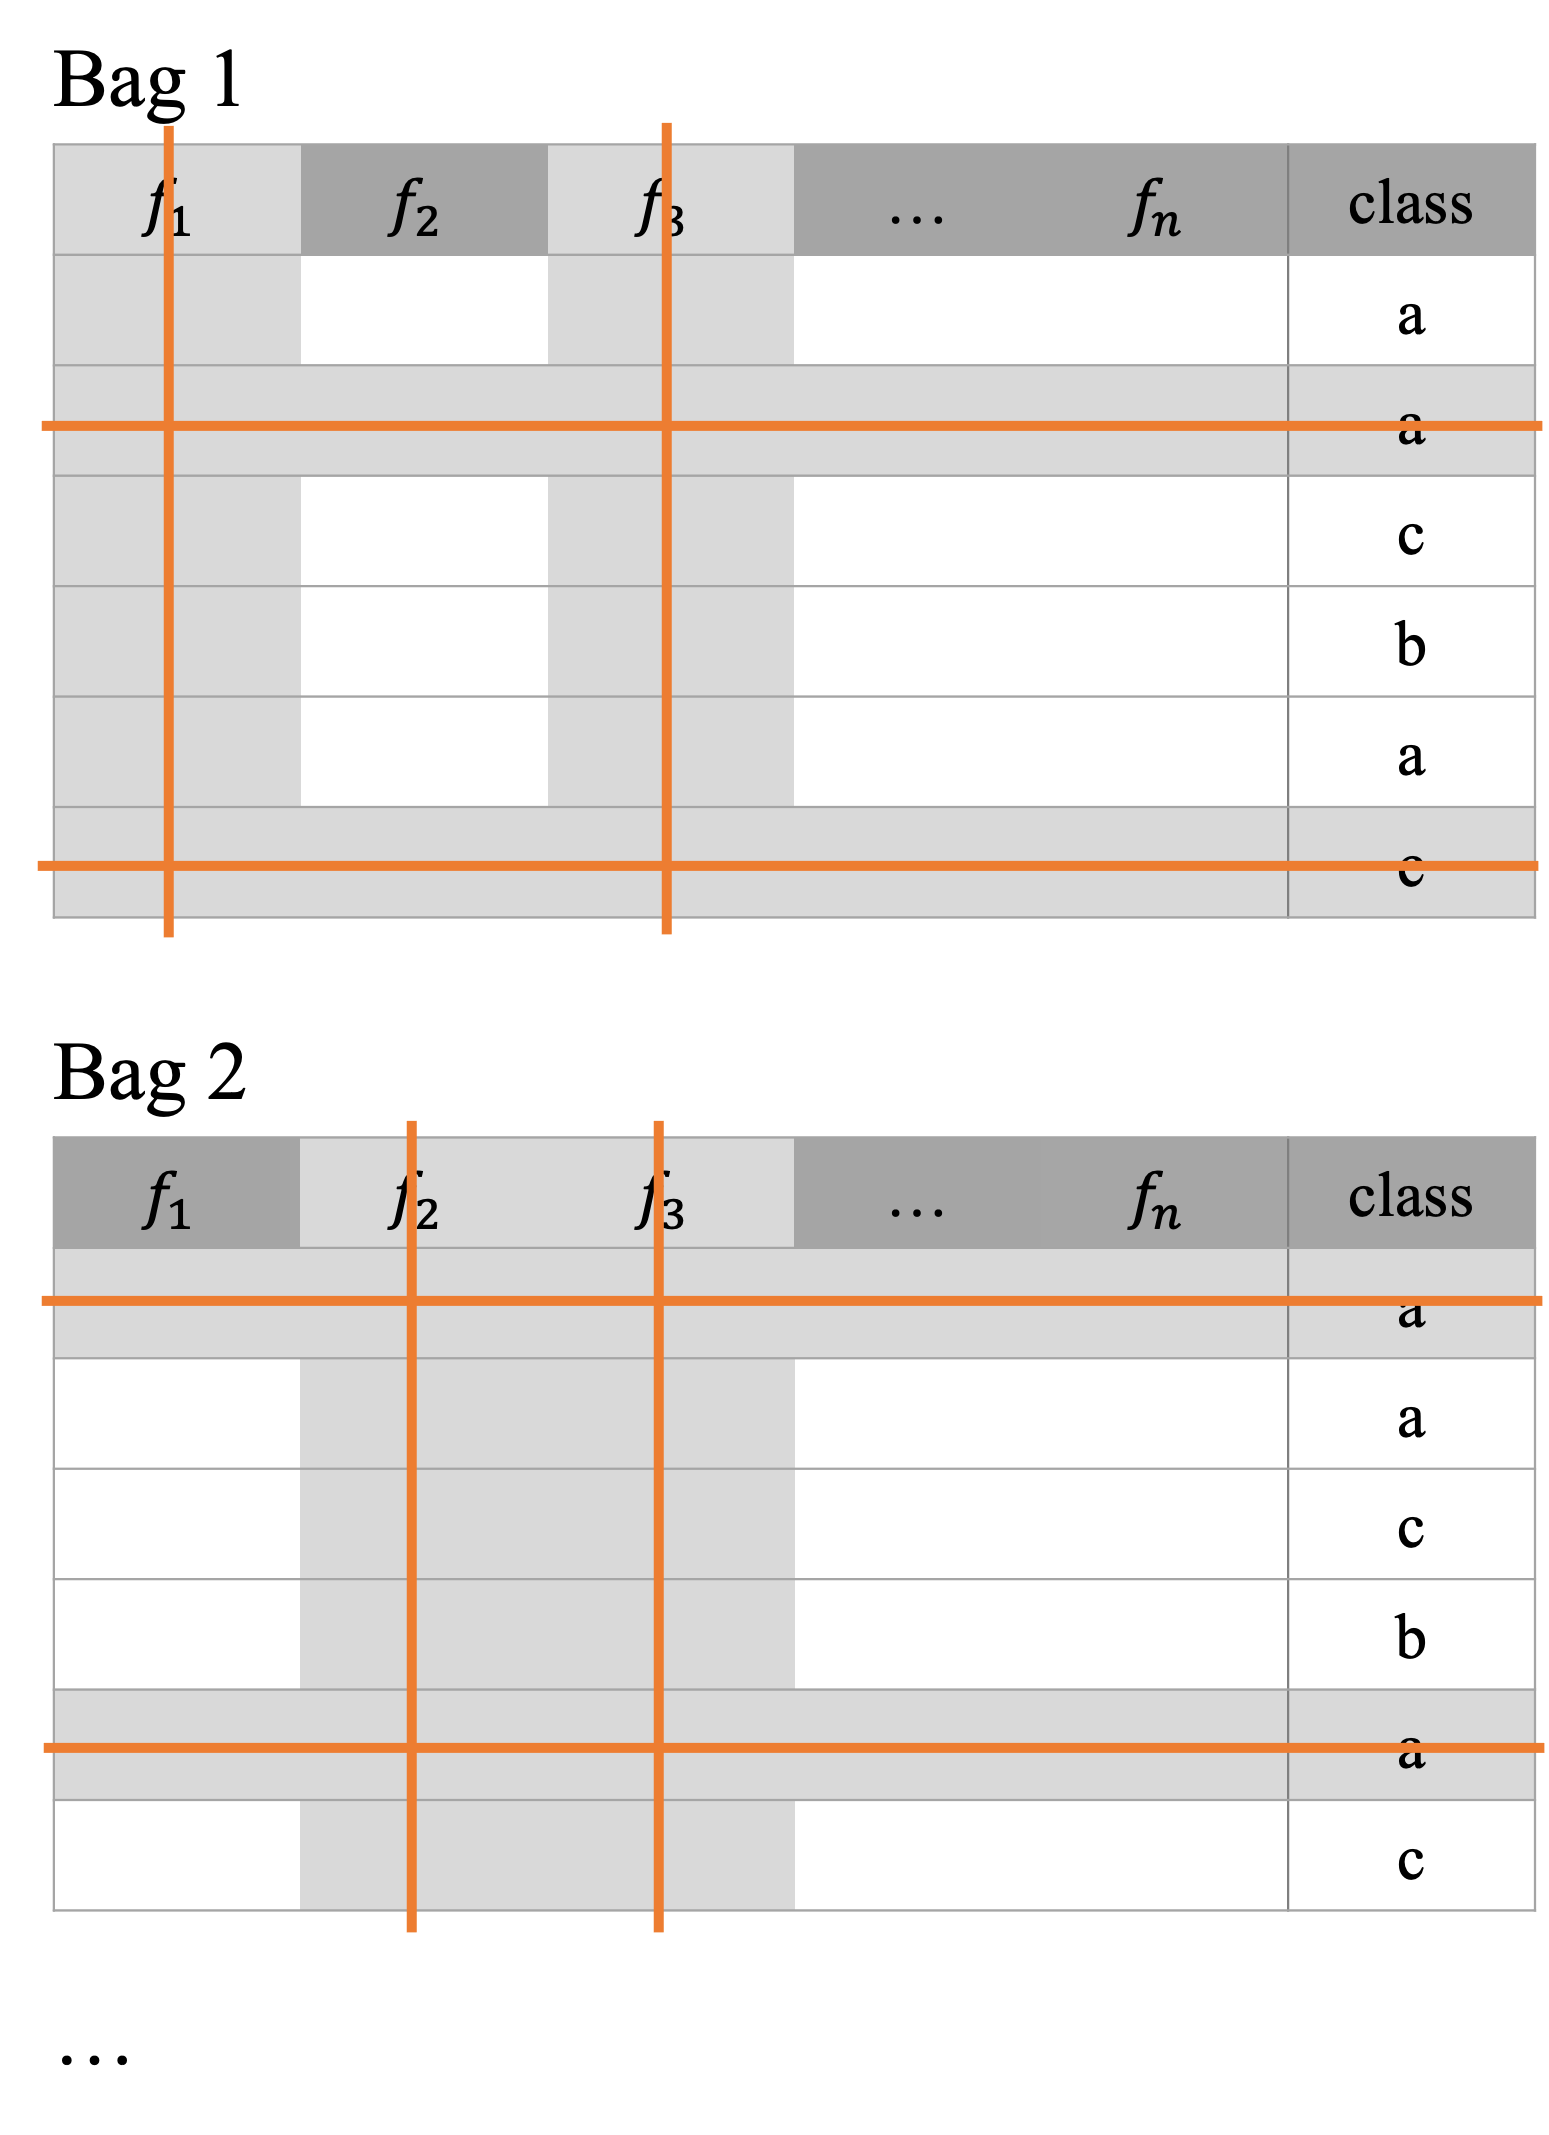
\includegraphics[width=0.9\textwidth]{assets/trees/id3/ensemble_comb_bagging.png}
    \subcaption{Random forest}
  \end{subfigure}
  \caption{Differnt ensemble bagging implementations}
  \label{fig:3_bagging}
\end{figure}

Finally, all of the ensemble methods can be combined in many possible combinations. 
\begin{itemize}
  \item When we have multiple classifiers (e.g. implemented as decision trees), they can be combined by voting or averaging.
  \item This often leads to a higher accuracy on unseen data and avoids overfitting.
\end{itemize}
